\insertmeeting 
	{Team Picture Day} 
	{09/15/22}
	{Hagerty High School}
	{Anouska, Jensen, Jorge, Karissa, Laura, Mohana, Nathan, Ritam, Robert, Samantha, Tyler}
	{Images/RobotPics/robot.jpg}
	{2:30 - 4:00}
	
\hhscommittee{General}
\noindent\hfil\rule{\textwidth}{.4pt}\hfil
\subsubsection*{Goals}
\begin{itemize}
    \item Work on linear slides prototype on CAD
    \item Divvy up hardware tasks
    \item Take team photos

\end{itemize} 

\noindent\hfil\rule{\textwidth}{.4pt}\hfil

\subsubsection*{Accomplishments}
We came to this meet looking our best today, as we are taking team photos. We came in the uniforms we would be wearing at our meets; a buttoned black shirt, black pants, as well as ties, buttons, bows, bandanas, and other extra clothing items courtesy of the program. There was a bit of waiting time before it was time, so our hardware committee worked on a Linear Slides System in CAD as a prototype. It’s for our current idea, which involves holding a rotating arm that is placed on a vertical linear slide, placed on a horizontal linear slide. 

Once everybody was ready we went down to our school's local amphitheater to take team photos and individual photos. The team photos would be for our school's yearbook, website, and socials, while the individual photos would be posted to the team section of our website. Now that our multimedia people have everything they need to make their first update to the website for the season, they will be getting to work very soon.

Hardware also had an important moment here. After taking photos, our hardware committee met up to divvy up work for different parts of the robot for the season. This plan is very important to us, as otherwise it is possible some may be left without work, or some may feel pressured and do too much. It also helps with accountability, since having each person confirm a role is far more likely to get it done than if it's simply put out there for the taking. Hopefully, with this new plan can make for a fair and efficient work environment for the hardware committee.


\begin{figure}[htp]
\centering
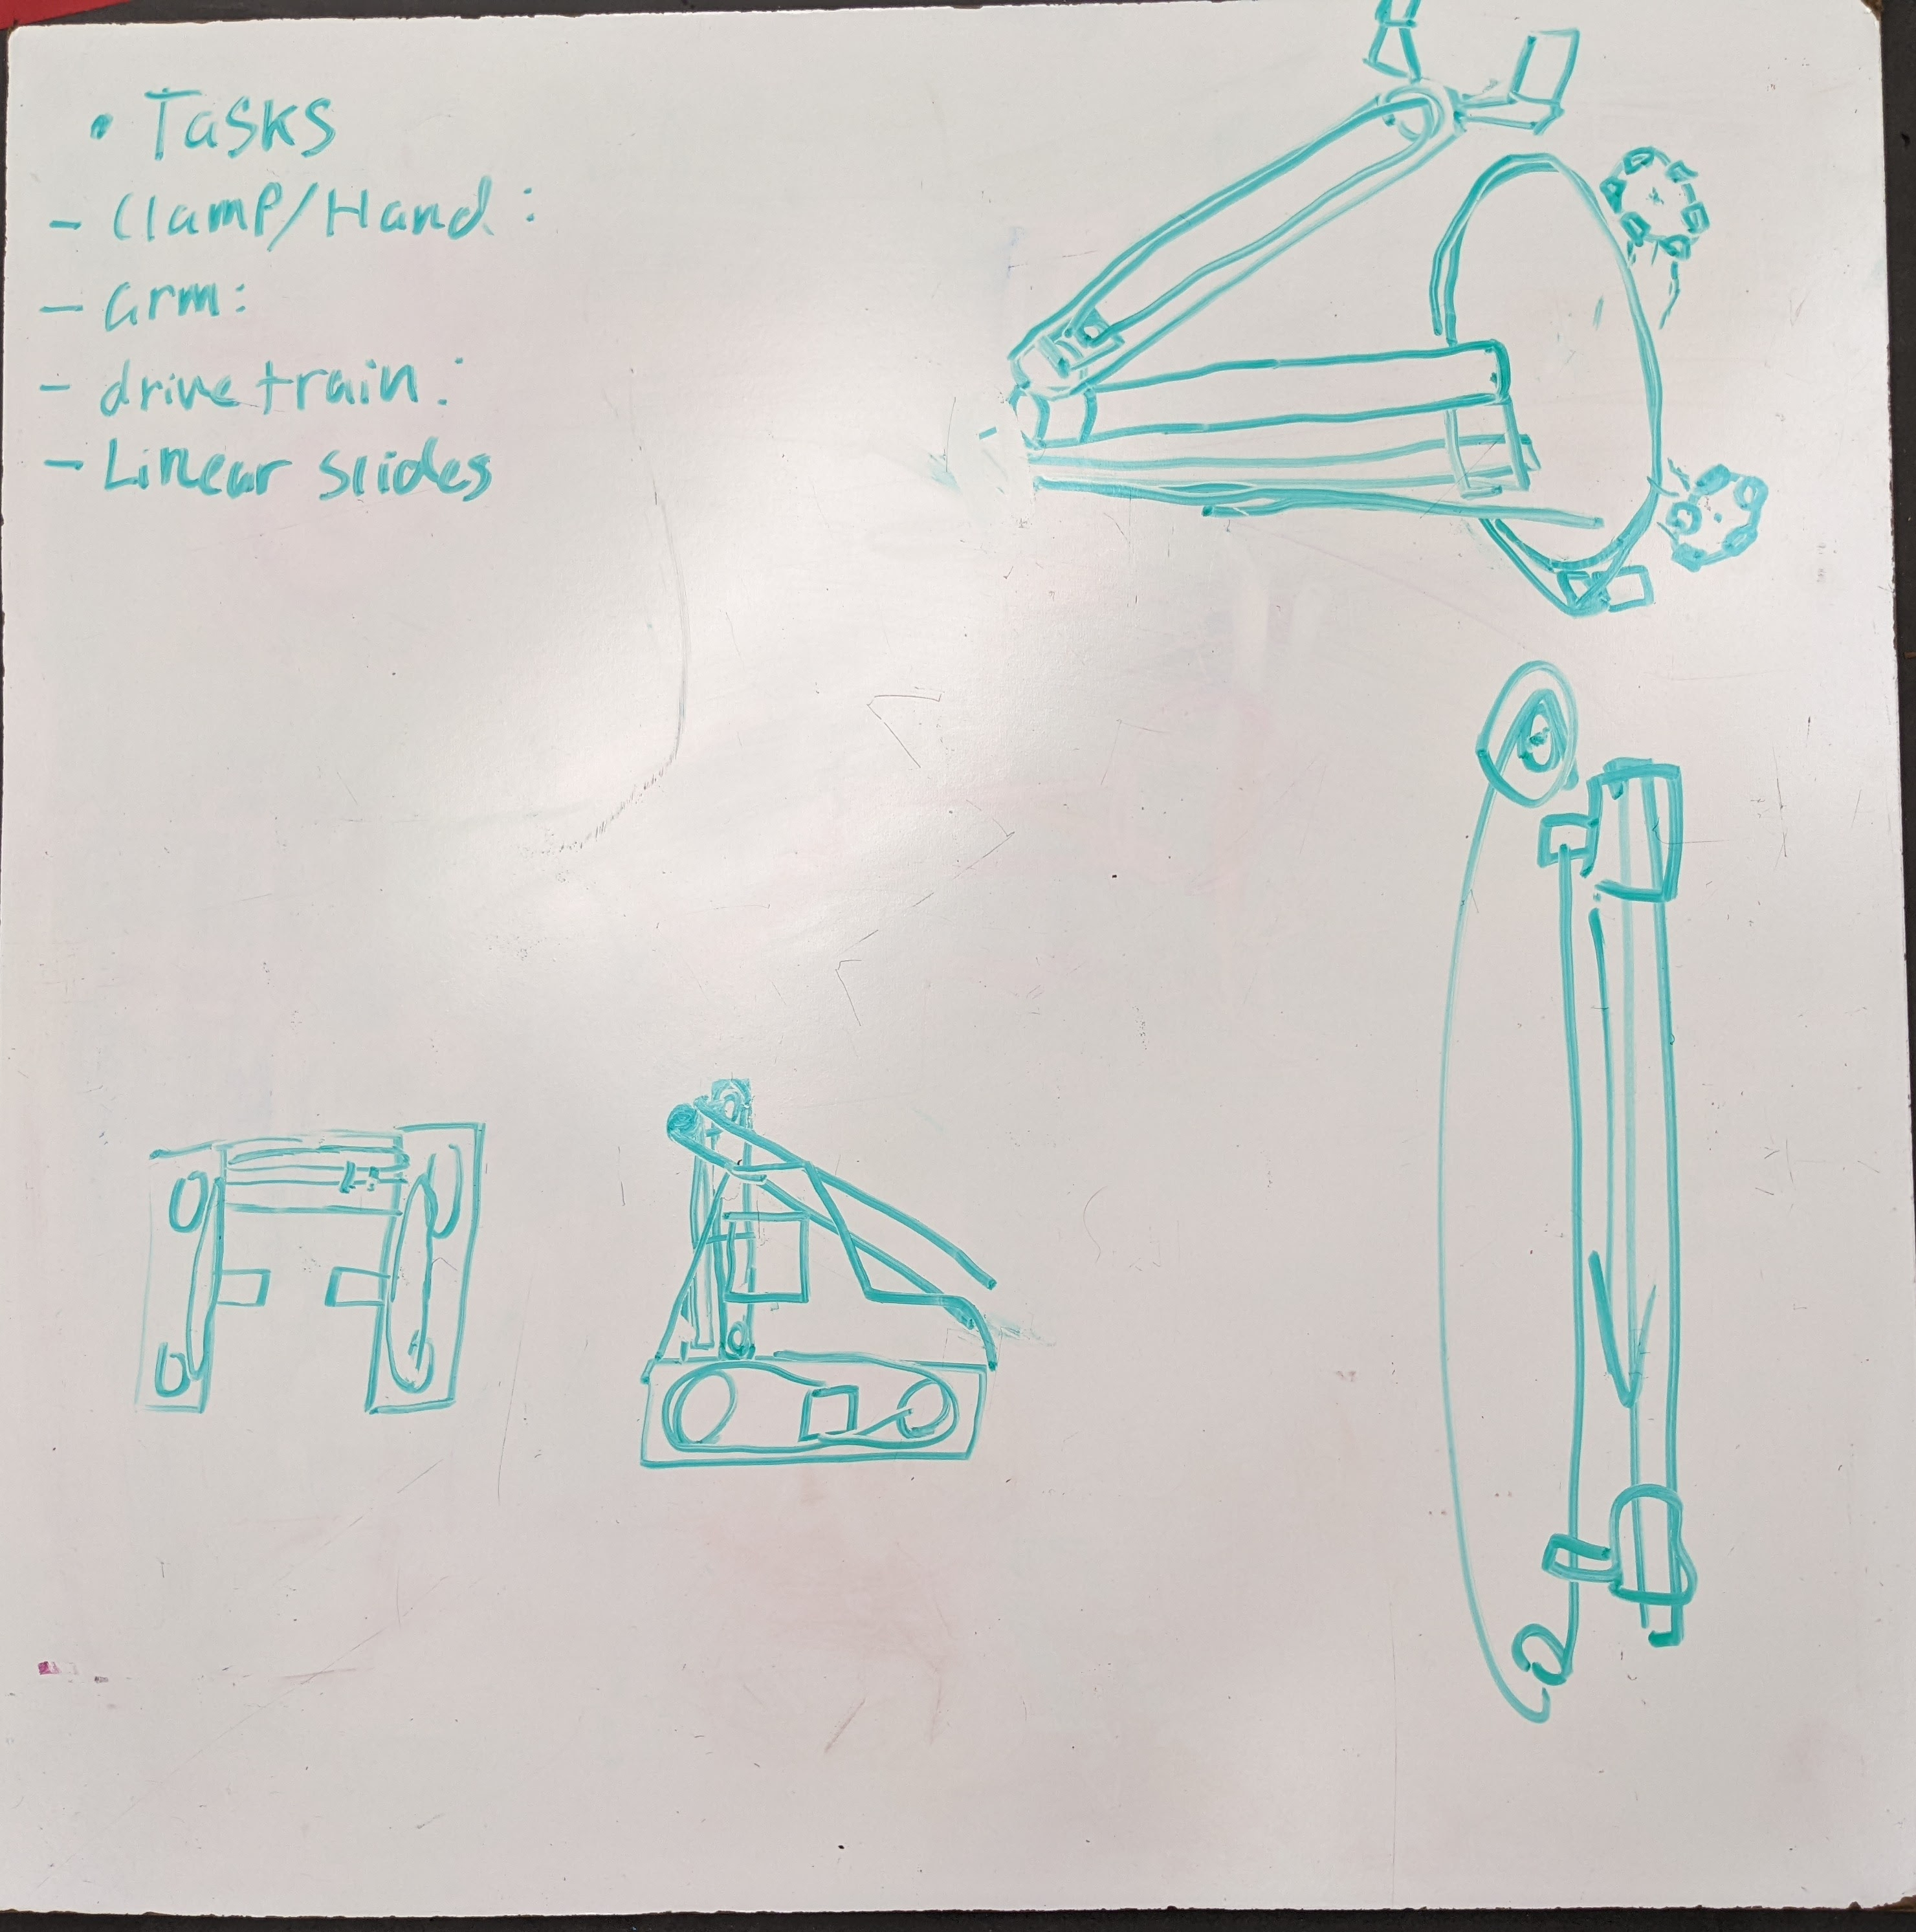
\includegraphics[width=0.95\textwidth, angle=0]{Meetings/September/09-15-22/09-15-22-Hardware.jpg}
\caption{List of possible hardware mechanisms}
\label{fig:pic3}
\end{figure}

\begin{figure}[htp]
\centering
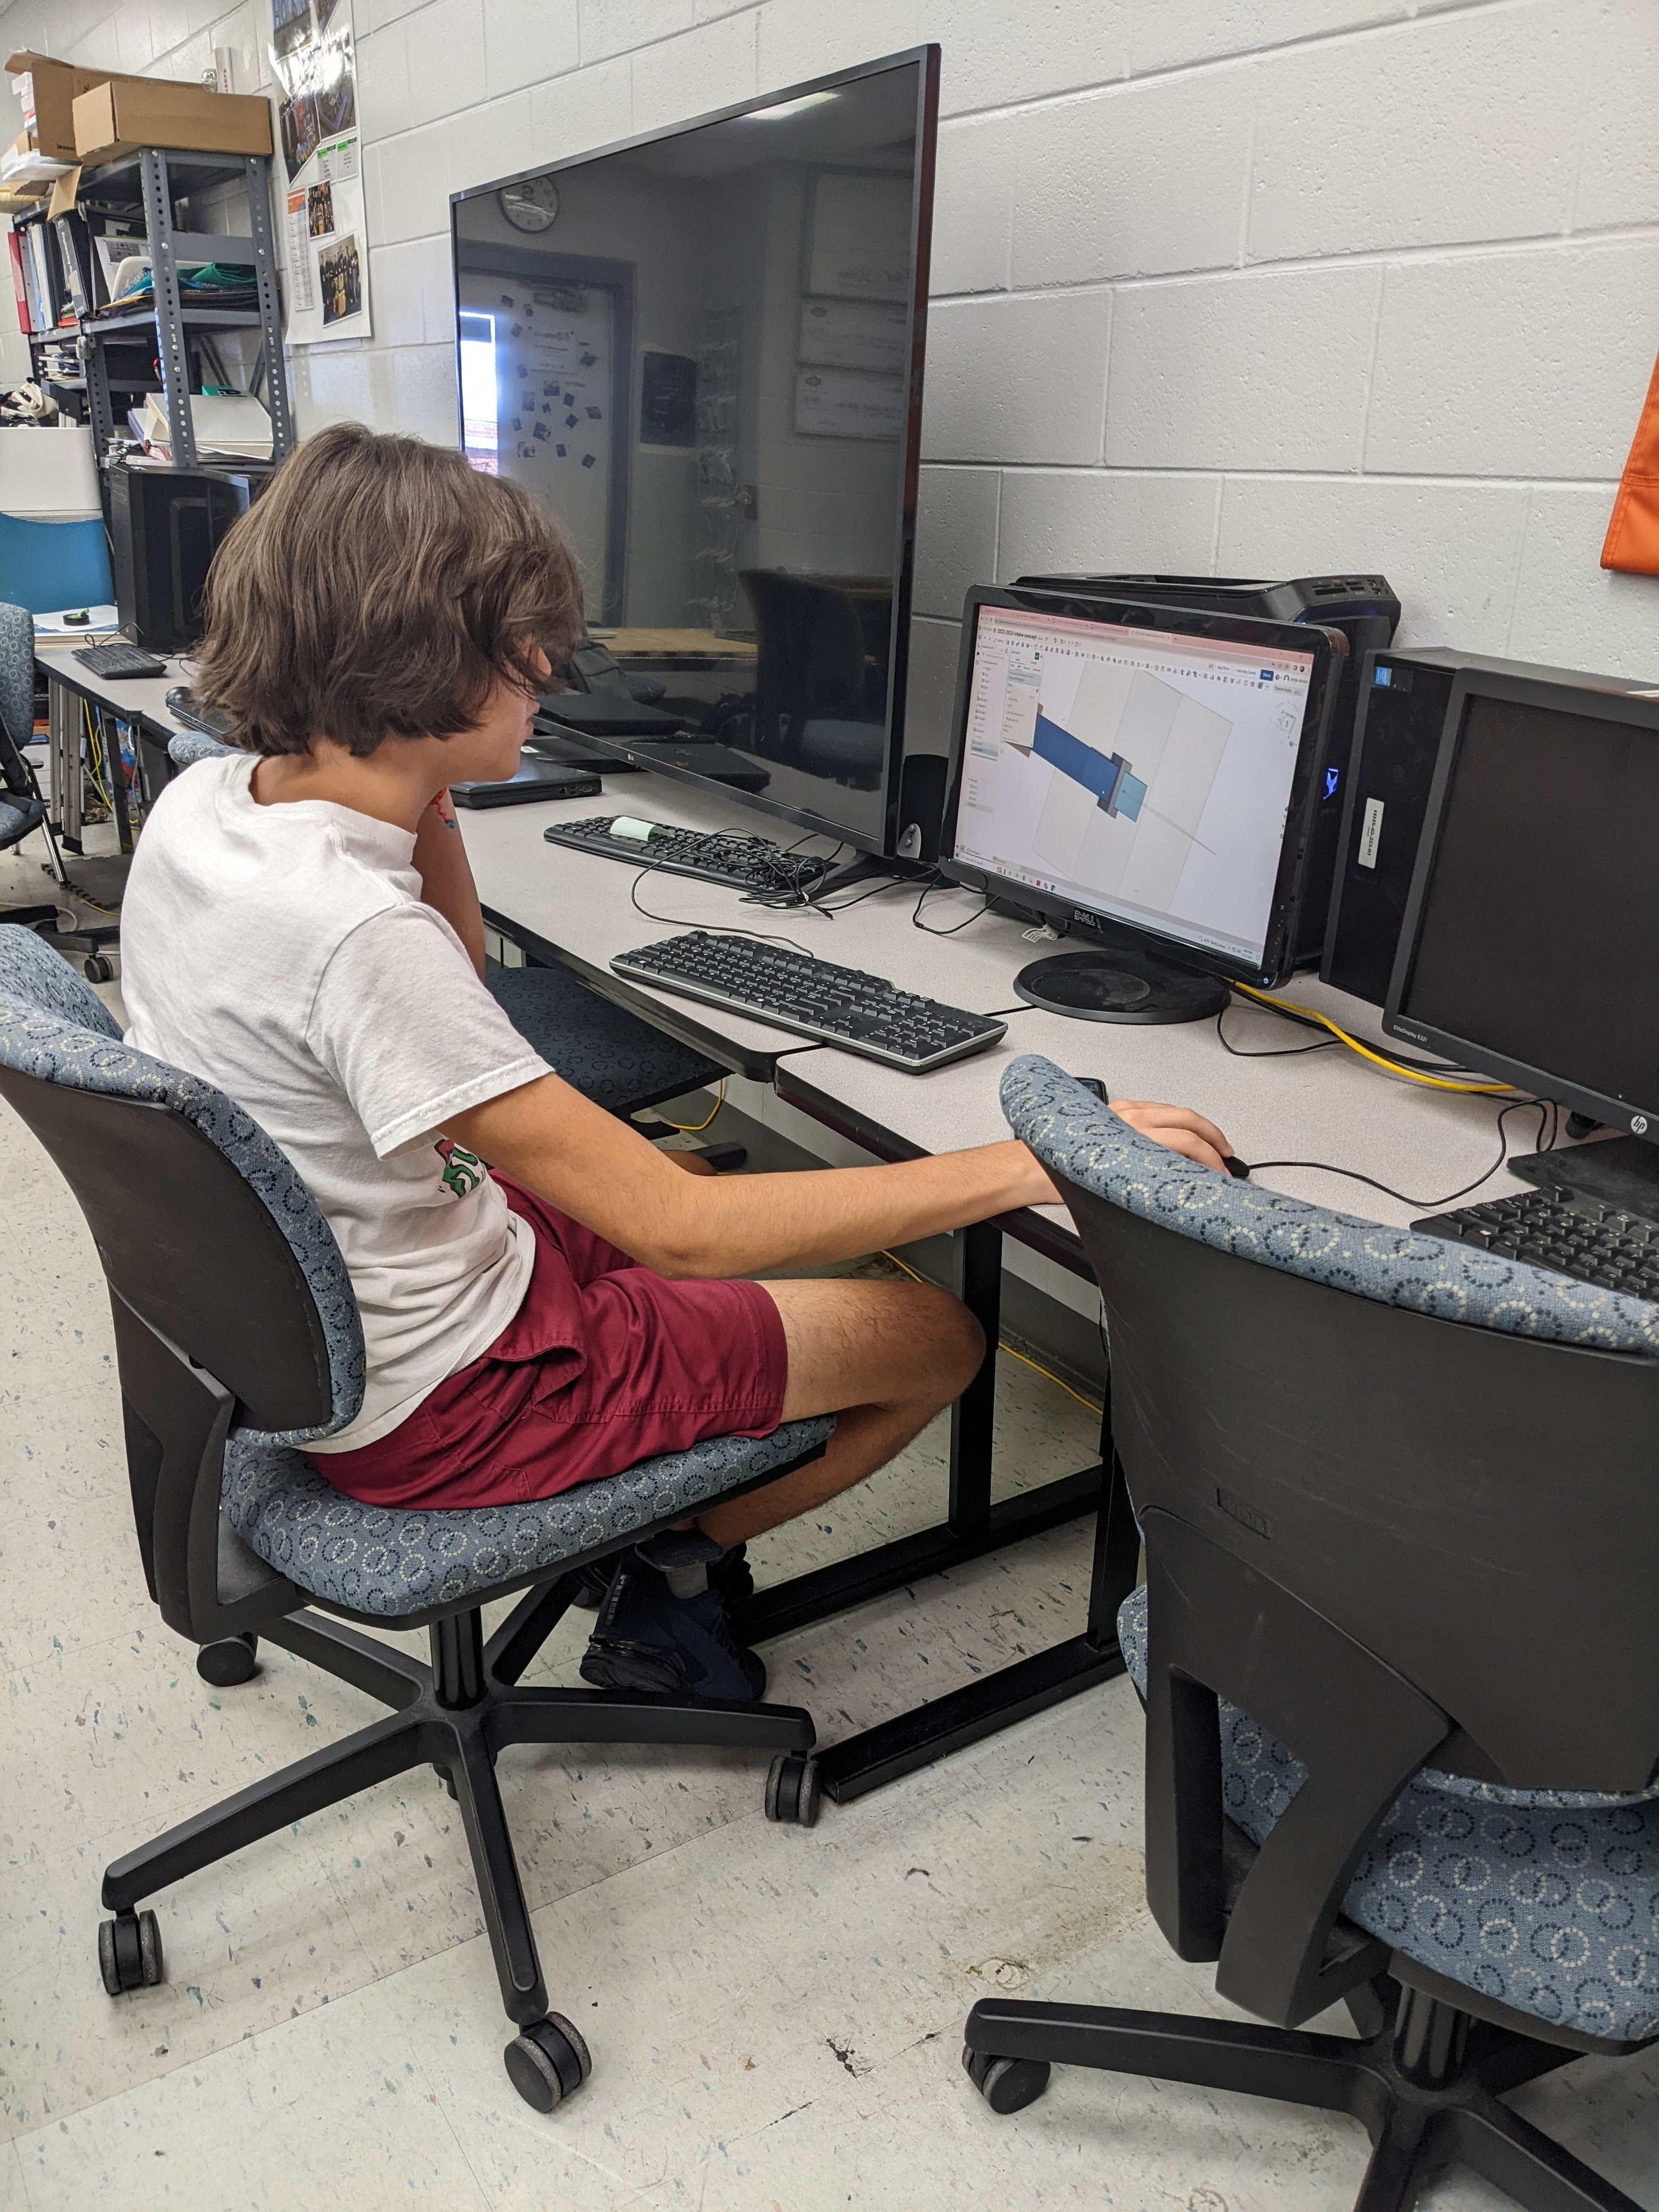
\includegraphics[width=0.95\textwidth, angle=0]{Meetings/September/09-15-22/09-15-22-meeting.jpg}
\caption{Working on comuter-aided design in Onshape}
\label{fig:pic3}
\end{figure}


% \begin{figure}[htp]
% \centering
% 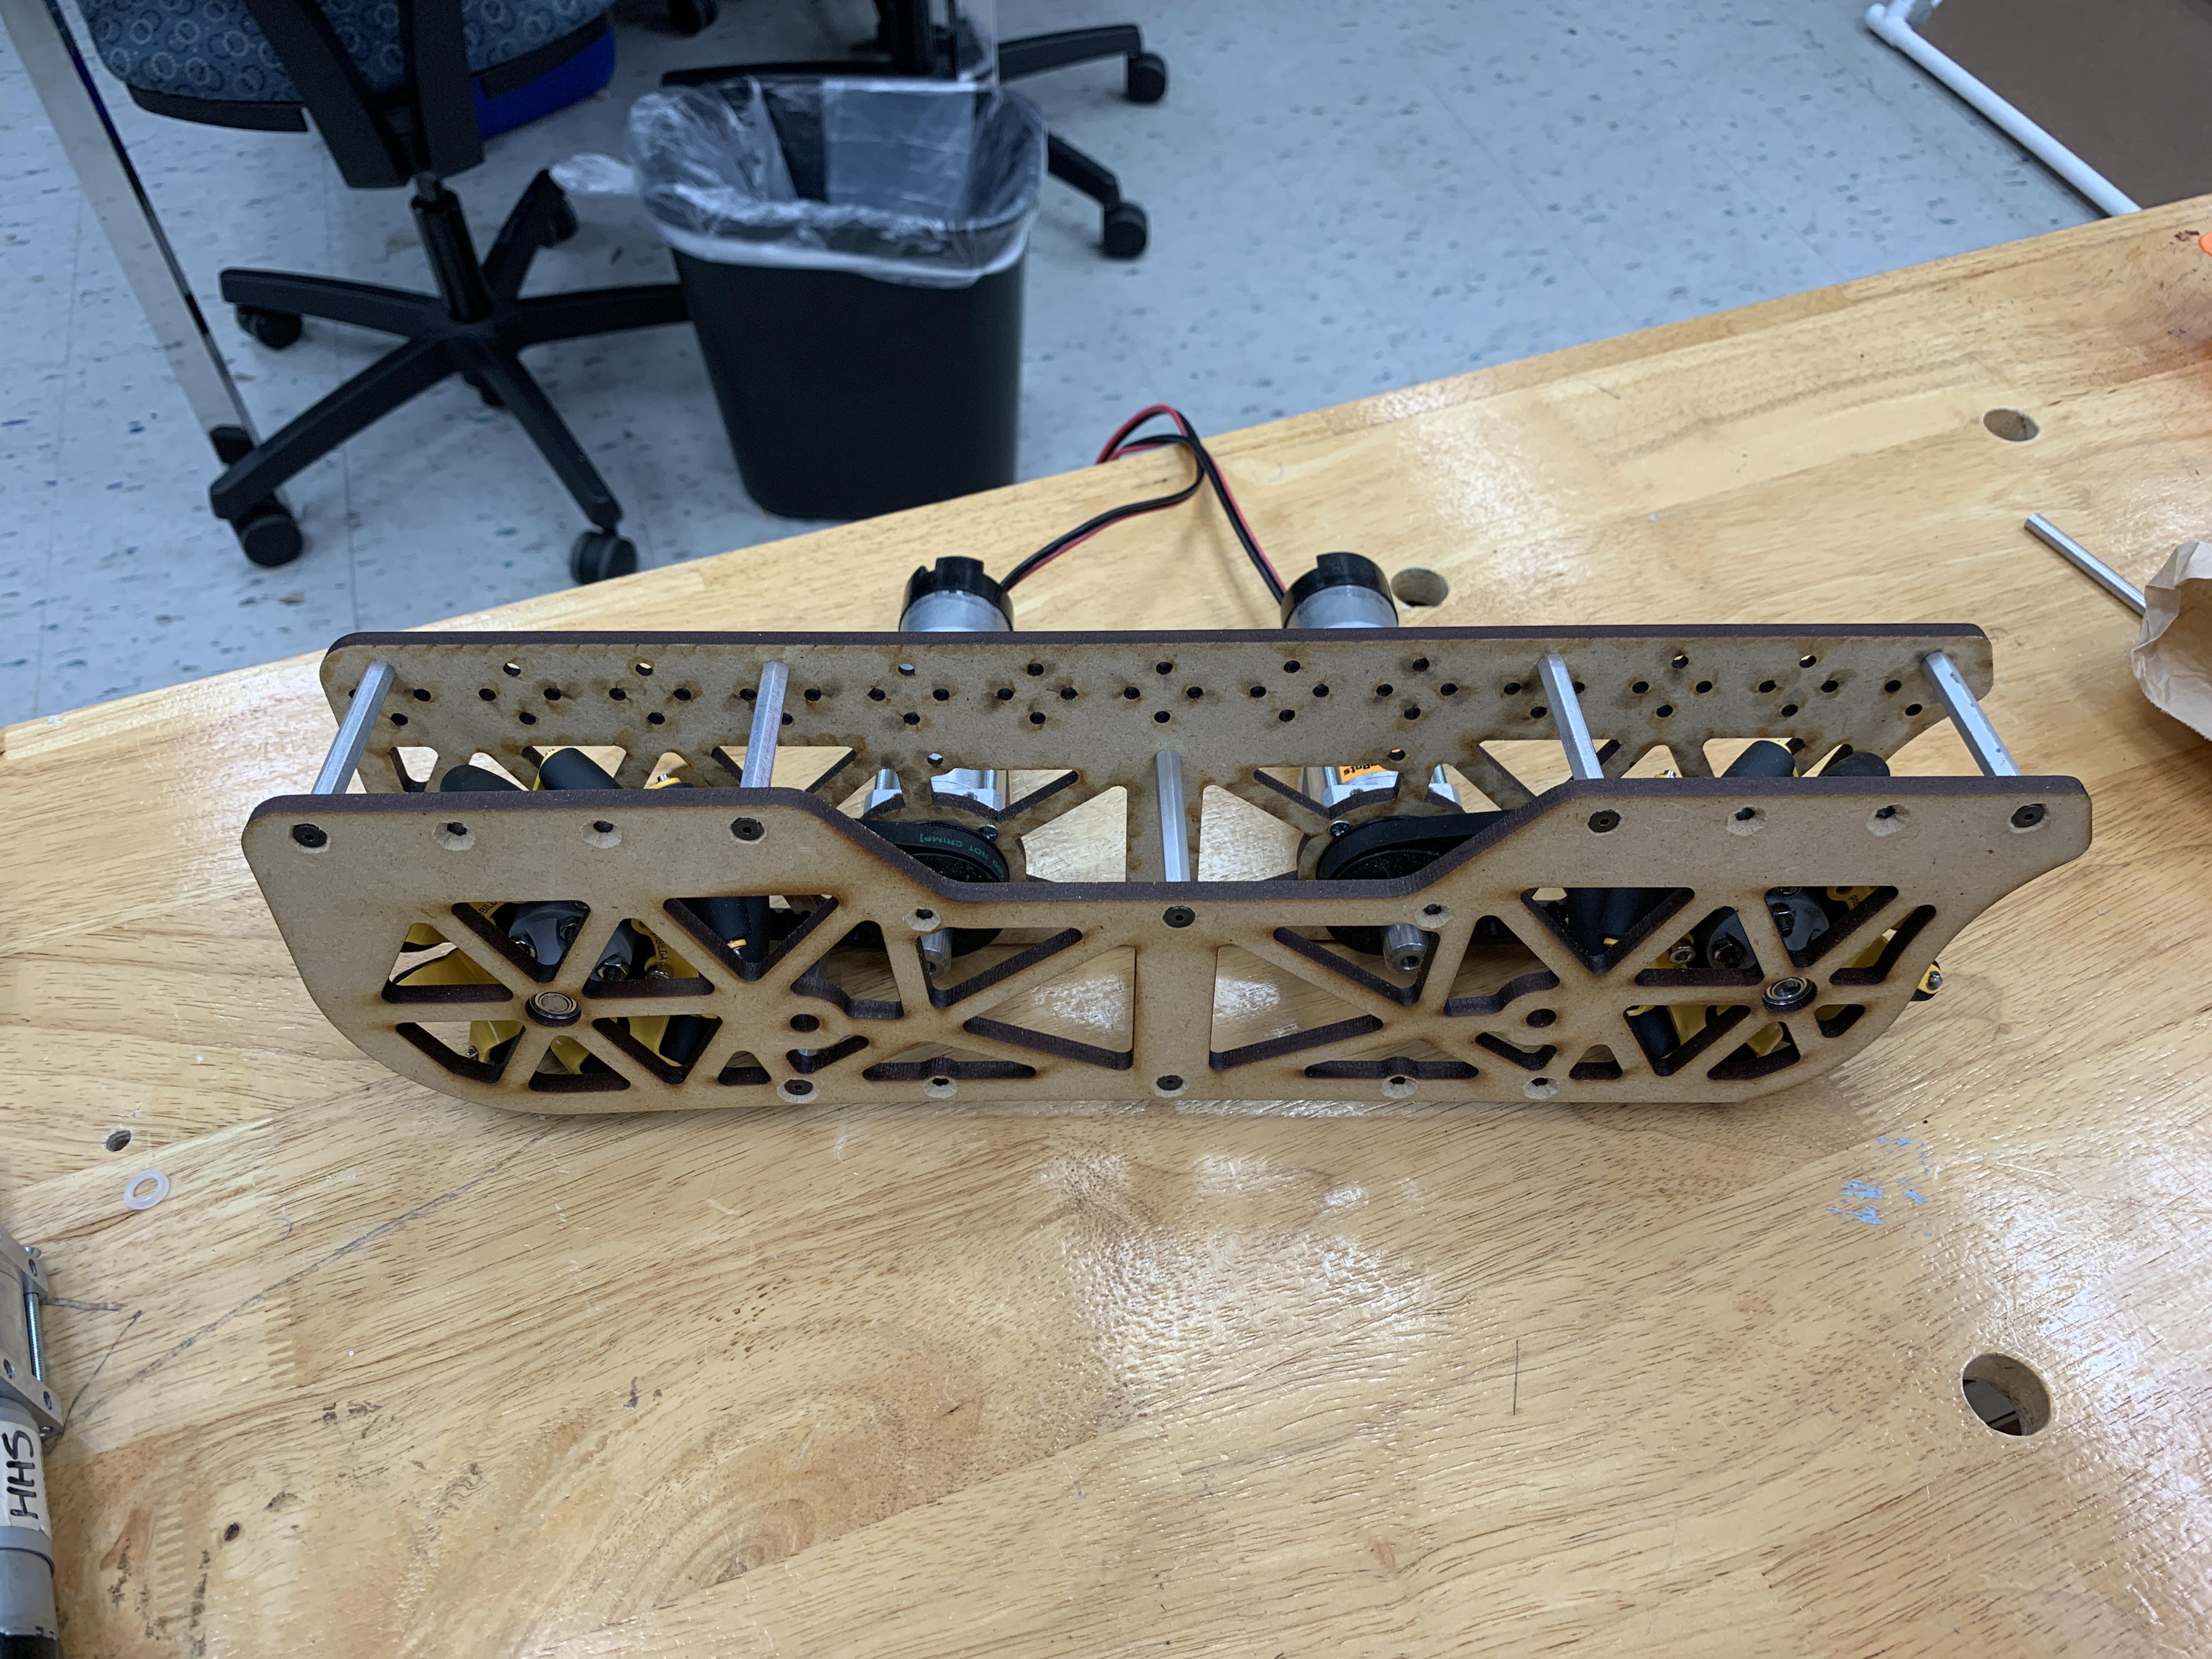
\includegraphics[width=0.9\textwidth, angle=0]{Meetings/July/07-21-21/drivetrain_7-20-21-NathanForrer.jpg}
% \caption{First half of the drivetrain.}
% \label{fig:072121_1}
% \end{figure}

\whatsnext{
\begin{itemize}
    \item Start working on signal sleeve for autonomous
    \item Test the signal sleeve prototypes
    
\end{itemize} 
}
